We ran one forward pass per response over the prompt followed by the model's own greedy output, cut shortly
after the harmful item's answer begins. At three positions we record the projection
$\langle h_\ell,\dhat_\ell\rangle$: the last prompt token; the first content token of the harmful item's
answer, the \emph{answer onset}; and the answer onset of the nearest benign item. We use 200 harmful targets
for each $k\in\{0,3,15\}$ $\times$ \{first, last\}, plus the benign-target controls. Responses that refuse the
item up front have no harmful answer onset and are excluded from onset statistics. \Cref{tab:probe} reports
the selected layer, and \cref{fig:auc} shows every layer.

\begin{table}[t]
\centering\small
\caption{Projection onto the refusal direction at the selected layer (Qwen3-14B: 36; Gemma-2-9B:
\GemmaLayer; Llama-3.1-8B: \LlamaLayer). Values are means; AUCs compare item-refused and item-complied responses
to list prompts (800 probed list responses per model, of which 39, 11 and 54 complied; Gemma's AUCs therefore
rest on few positives). The last rows split list responses by the sign of the last-token projection.}
\label{tab:probe}
\resizebox{\linewidth}{!}{\begin{tabular}{lccc}
\toprule
Projection (\% of harmful-alone value) & Qwen3-14B & Gemma-2-9B & Llama-3.1-8B \\
\midrule
last prompt token, harmful request alone & +100 & +100 & +100 \\
last prompt token, benign request alone & -30 & +4 & -6 \\
\midrule
last prompt token, harmful item first & +30 & +60 & +15 \\
last prompt token, harmful item last & +11 & +40 & +20 \\
\midrule
harmful item's answer onset, item refused & +4 & +56 & +27 \\
harmful item's answer onset, item complied & -18 & +35 & +29 \\
benign item's answer onset & -25 & +10 & +6 \\
\midrule
AUC refused vs.\ complied, answer onset (sel.\ / best layer) & 0.88 / 0.91 (27) & 0.86 / 0.90 (26) & 0.46 / 0.83 (16) \\
AUC refused vs.\ complied, last prompt token (sel.\ / best) & 0.95 / 0.95 (24) & 0.92 / 0.97 (38) & 0.69 / 0.91 (25) \\
\quad control: same request \emph{alone}, last prompt token (layer) & 0.95 (24) & 0.89 (38) & 0.93 (25) \\
\midrule
lists with negative last-token projection & 16\% & 0\% & 3\% \\
\quad ASR / target refused, if negative & 23\% / 46\% & -- & 23\% / 55\% \\
\quad ASR / target refused, if positive & 1\% / 95\% & 1\% / 97\% & 6\% / 86\% \\
\bottomrule
\end{tabular}}
\end{table}

\paragraph{Lists shrink the last-token read-out and flip its sign, but not its ranking.} A harmful request
alone gives a large positive projection at the last prompt token, and a benign request a small or negative one
(\cref{tab:probe}; values are scaled so that harmful-alone $=100$). Embedding the harmful request in a list
shrinks the last-token projection to 11--60\% of that value. For Qwen3-14B it turns negative in
\QwenNegLastFrac\ of list prompts, which is the ``sign flip'' of our earlier study. Llama-3.1-8B flips in
\LlamaNegLastFrac\ of list prompts and Gemma-2-9B never does. Read naively, a negative
projection says the model has moved into the non-refusal half-space. Behaviourally that reading is wrong most
of the time: when the sign flips, the model still refuses the harmful item or deflects it in about 77\% of
responses in both Qwen3-14B and Llama-3.1-8B. It is right about risk, though: ASR is 23\% when the sign flips
and 1--6\% when it does not.

The ranking survives the shift. Within list prompts, the last-token projection separates responses that end up
refusing the harmful item from those that comply, with AUC up to \QwenAUCLastBest\ (Qwen3-14B),
\GemmaAUCLastBest\ (Gemma-2-9B) and \LlamaAUCLastBest\ (Llama-3.1-8B) at the best layer (\cref{fig:auc}). So the end of the prompt already encodes
what the model will do \emph{when it gets to} the harmful item, even though its first output tokens are about
something else. What breaks is the \emph{calibration} that maps the projection to the next tokens. The zero
point that separates refusal from compliance for single requests does not carry over to lists. Last-token
probes are not wrong about the model's state; they are wrong about \emph{when} that state takes effect.

\paragraph{The same information is present at the item.} At the harmful item's answer onset, the projection
separates refused from complied items with AUC up to \QwenAUCOnsetBest\ (Qwen3-14B), \GemmaAUCOnsetBest\
(Gemma-2-9B) and \LlamaAUCOnsetBest\ (Llama-3.1-8B), slightly below the last-token values. It also sits clearly above the answer onsets of benign items in the same responses
(\cref{tab:probe}). In all three models the separation appears only in later layers: from about layer 20 of 40 in Qwen3-14B,
layer 20 of 42 in Gemma-2-9B and layer 12 of 32 in Llama-3.1-8B. For Llama-3.1-8B it is weak at the causally selected layer 10
(\cref{tab:probe}). Absolute projections at the onset are small compared with the harmful-alone value, which is
expected, since $\dhat$ was fit at last-prompt-token positions of single requests.

\paragraph{The ``guardrail head'' looks when it needs to.} Our earlier study reported that Qwen3-14B's head
L36H31, the largest direct contributor to $\dhat_{36}$, loses attention to the harmful request under dilution.
From the last prompt token of a list prompt, its attention mass on the harmful request's tokens is indeed
small: \AttnLast, against \AttnBare\ for the request alone. From the harmful item's answer onset it is
\AttnOnset, several times higher than from the last prompt token and higher than the mass the same head puts on
a benign item's own request at that item's onset (\AttnBenignOwn). The head reads whichever request the model
is currently answering. Its low attention from the last prompt token reflects \emph{where we measured}, not a
lesion.



\begin{figure}[t]
\centering
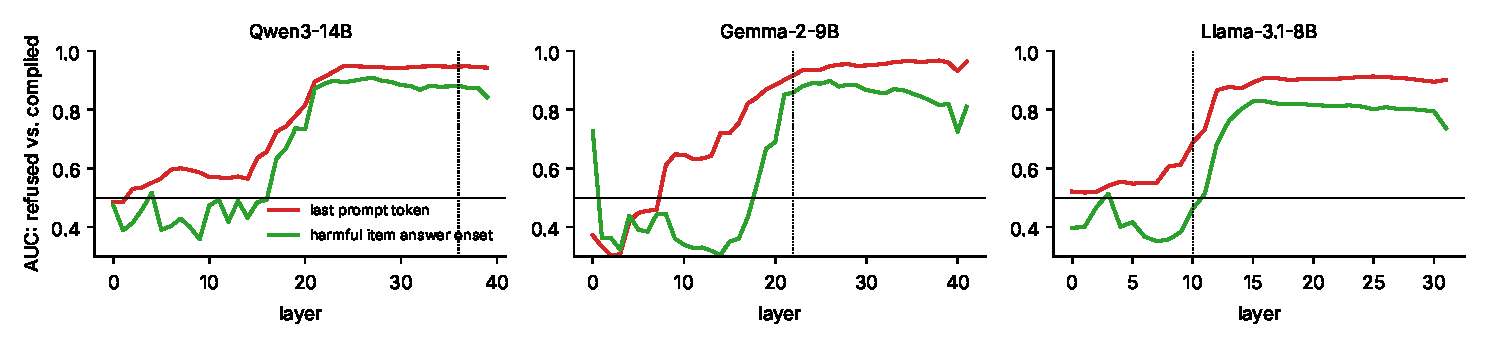
\includegraphics[width=\linewidth]{generated/fig_auc_layers.pdf}
\caption{How well the projection onto $\dhat_\ell$ separates list responses that refuse the harmful item from
those that comply (HarmBench), by layer. Red: read at the last prompt token. Green: read at the harmful item's
answer onset. Dotted: causally selected layer.}
\label{fig:auc}
\end{figure}
